%% osm-communaute.tex


\section{Communauté}

\frame[plain]{  \heading{Plan de la Présentation}
\ecmsetupplan
\begin{itemize}
  \item[\small $\Diamond$] Introduction
  \item[\small $\Diamond$] Fonctionnement 
  \item[\small $\Diamond$] Applications
  \item[\small $\Diamond$] Technique
  \item[\small $\Diamond$] {\color{purple}\textbf{Communauté}}
  \item[\small $\Diamond$] Conclusions
\end{itemize}
}

%% http://www.microsoft.com/presspass/exec/billg/speeches/2006/03-20MIX.mspx
\frame{\heading{Une citation} \vfill

  \begin{changemargin}{2cm}{2cm}
 \begin{tikzpicture}[overlay]
   \node [xshift=-1.1cm,yshift=-0.5cm] 
      [font={\fontfamily{ptm}\fontsize{105}{105pt}\selectfont\color{blue!40}}]{`\kern-0.1em`};
   \end{tikzpicture}
{\sl You could have a community capability where you took the GPS data of
people driving around and started to see, oh, there's a new road that
we don't have, a new route... And so that data eventually should just
come from the community with the right software infrastructure.

\bigskip

\pause
\hfill Bill Gates\\
\hfill Conférence MIX06\\
\hfill Las Vegas, mars 2006} %
   
\begin{tikzpicture}[overlay]
     \node [xshift=0.8cm,yshift=-0.6cm] 
       [font={\fontfamily{ptm}\fontsize{76}{76pt}\selectfont\color{blue!40}}]{'\kern-0.1em'};
   \end{tikzpicture}
   \end{changemargin}
}


%% http://wiki.openstreetmap.org/wiki/Stats
\frame{ \heading{Croissance?} \vfill
  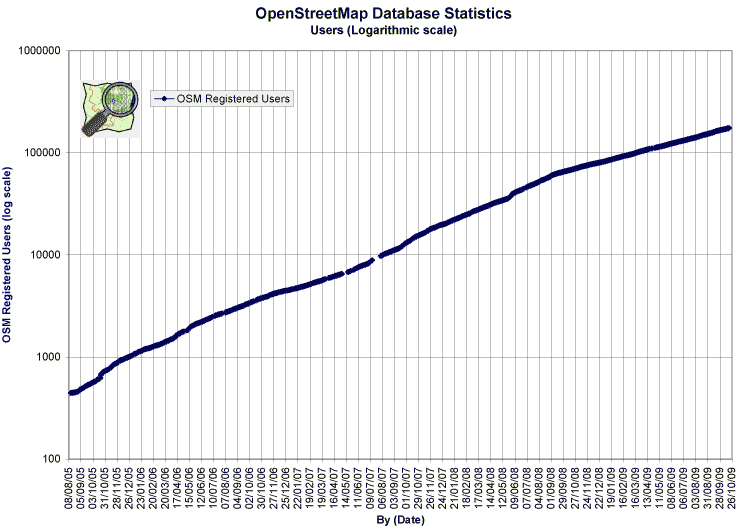
\includegraphics[width=0.95\textwidth]{figures/Osmdbstats1_log}
}

\frame{ \heading{Croissance?} \vfill
  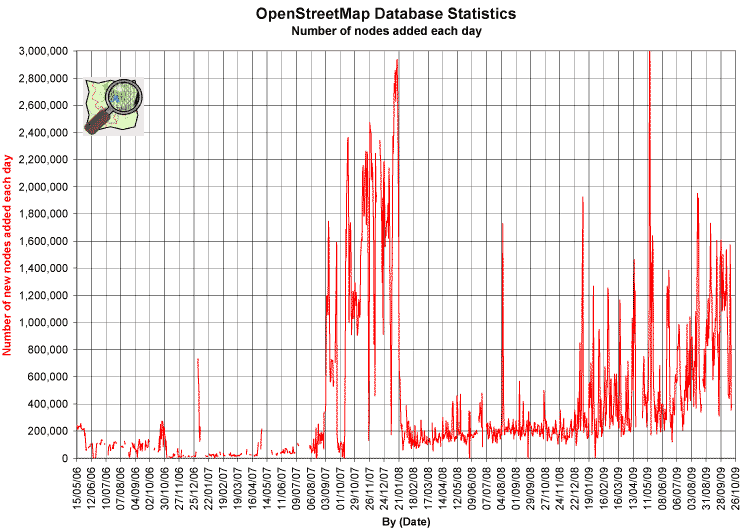
\includegraphics[width=0.95\textwidth]{figures/Osmdbstats7A}
}



\frame{\heading{Pourquoi ça marche?} \vfill

 \begin{itemize}
 \item Données collectées avec des GPS très variables en qualité

 \item Contributeurs de nombreuses cultures, parlant des langues
   différentes, ayant des centres d'intérêt différents

 \item Chacun peut tagguer comme il l'entend (``free-form'', ni schéma
   homogène ni police)

 \item Système de vote wiki pour les nouveaux tags, ignoré par
   certains («~on vote en utilisant le tag~»)

 \item Mécanismes de protection contre le vandalisme très primitifs
 \end{itemize}
}


%% EOF
